\documentclass[11pt,a4paper]{article}

\usepackage[T1]{fontenc}
\usepackage[utf8]{inputenc}
\usepackage{lmodern}
\usepackage[margin=2cm]{geometry}
\usepackage{amsmath}
\usepackage[round]{natbib}
\usepackage{xcolor}
\usepackage[colorlinks=true,linkcolor=blue!60!black,citecolor=blue!60!black,urlcolor=blue!60!black]{hyperref}
\usepackage{tikz}
\usepackage{titlesec}
\usepackage{multicol}
\usepackage{graphicx}
\usepackage[font=small,labelfont=bf,labelsep=colon]{caption}

\titleformat{\section}{\large\bfseries}{}{0pt}{}
\titlespacing*{\section}{0pt}{10pt}{4pt}
\setlength{\parskip}{4pt}
\setlength{\parindent}{0pt}
\setlength{\bibsep}{0pt}

\newcommand{\desilike}{\texttt{desilike}}

\begin{document}

\begin{center}
{\Large\bfseries Statement of Research Interests}\\[4pt]
Dr.\ Federico D\'avila-Kurb\'an \;|\; \href{mailto:fdavilakurban@unc.edu.ar}{fdavilakurban@unc.edu.ar} \;|\; ORCID: 0000-0001-5612-6460
\end{center}

%=====================================================================
\section*{Overview}

I work on large-scale structure statistics, and my research has one consistent aim: to extract cosmological information from the galaxy distribution that standard two-point analyses do not capture, using the cosmic-web environment of galaxies as a lever. I combine N-body and hydrodynamical simulations with survey data, and I build and improve the statistical tools these studies require: Baryon Acoustic Oscillation (BAO) fits, covariance estimates, efficient correlation-function estimators and higher-order clustering statistics. I obtained my PhD in 2022 at the Universidad Nacional de C\'ordoba with a thesis on galaxies and structures in cosmic voids, and I have led most of my projects as first author. I currently carry out my research at the Instituto de Astronom\'ia Te\'orica y Experimental (IATE, C\'ordoba) and hold an Assistant Professor position at the Universidad Nacional de C\'ordoba.

At the Berkeley Center for Cosmological Physics (BCCP) I propose to test whether the geometry of the cosmic web, and not only its density, shapes the acoustic feature, and whether DESI can use that information to sharpen or to safeguard its distance measurements.

%=====================================================================
\section*{Prior and current research}

\textbf{Current work: BAO and the cosmic web (paper in preparation).} I lead a project at IATE that asks whether the BAO feature depends on cosmic-web environment, focusing on filaments. The nonlinear damping of the acoustic peak is driven by bulk flows that vary strongly between environments, so an environment-dependent BAO signal would be either a new handle on the standard ruler or a systematic that current analyses do not control. Previous work has used local density as the environment: the acoustic peak shifts and broadens differently around high- and low-density regions \citep{Neyrinck2018,Xu2025}, the recovered BAO scale is biased for samples selected by local density \citep{HernandezAguayo2020}, and in BOSS CMASS the peak shape and the accuracy of reconstruction vary with density while the distance scale stays consistent \citep{Blake2018}. My approach selects galaxies by their distance to filaments, a non-local measure of the cosmic web, while controlling for local density. I designed the project and built its pipeline. DisPerSE filaments \citep{Sousbie2011} and nearest-neighbour densities define environment-split samples, and each sample is compared with a random dilution of the full sample matched in number density, so that an environmental effect is not confused with a change in shot noise. I measure the correlation-function monopole and the power spectrum, build analytic Gaussian covariances from the measured spectra without assuming a bias model, and fit the dilation parameter, the damping scale and the detection significance with \desilike, using joint fits that account for the correlation between samples and Gaussian mocks to calibrate the significance of their differences, with a template-free Gaussian peak fit as a cross-check. The first paper is designed as a sequence of increasingly realistic tests: the MultiDark galaxy catalogue, a periodic box with known cosmology, isolates the physical effect; the Flagship galaxy mock, built on a light cone \citep{Castander2025}, adds redshift evolution and a survey-like geometry while the cosmology is still known; and SDSS galaxies bring the method to observations. Preliminary measurements in MultiDark hint at a narrower acoustic peak for galaxies near filaments (Fig.~\ref{fig:pipeline}), though about 10\% of density-matched random dilutions reach it by chance; the full analysis will establish whether filament membership changes the amplitude, width or position of the acoustic peak. I expect to submit this paper before the fellowship starts. This project is the starting point of the main line of my proposal: the same pipeline, measured in the frame of the filaments, is the basis of WP1--WP3.

\begin{figure}[h]
\centering
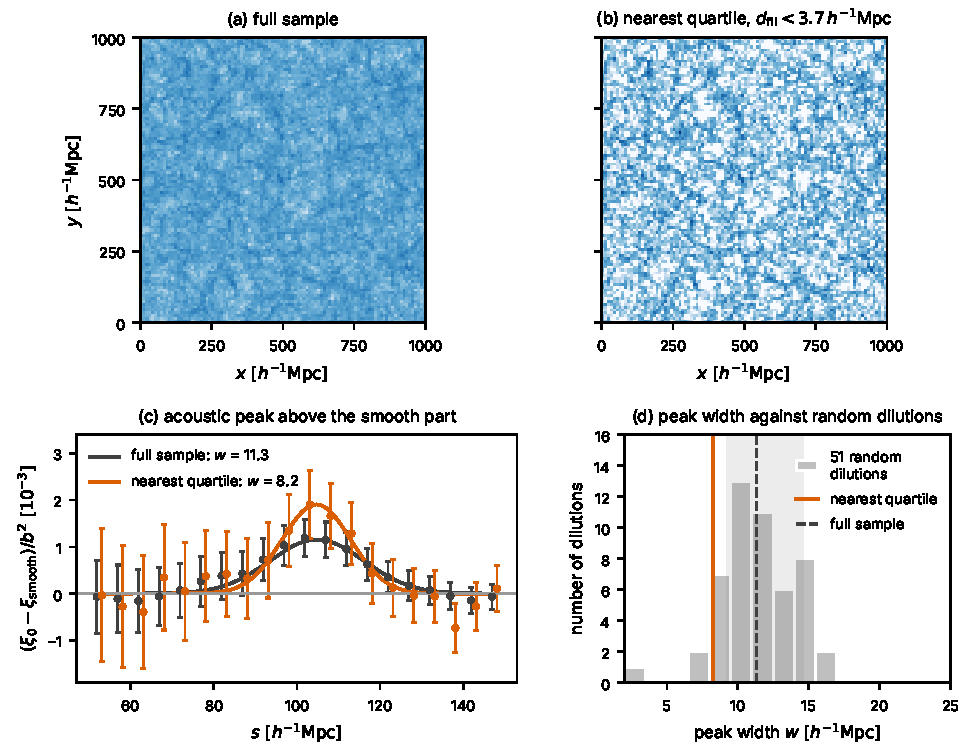
\includegraphics[width=0.77\textwidth]{fig_comparison.pdf}
\caption{Preliminary measurement in MultiDark (one simulation box, real space). (a, b) A 100\,$h^{-1}$Mpc slab of the full sample and of the quartile nearest to DisPerSE filaments (logarithmic galaxy counts per pixel). (c) Monopole minus its fitted smooth part, divided by $b^2$, with fitted Gaussians of width $w$. (d) Width $w$ of the nearest quartile against 51 random dilutions of the full sample with the same $N$ (shaded: 16--84\%). About 10\% of the dilutions have a peak at least as narrow, so the difference is not yet significant. \desilike\ template fits agree: lower damping for the nearest quartile than for its dilution ($\Delta\chi^2\simeq3$ for no difference).}
\label{fig:pipeline}
\end{figure}

\textbf{Higher-order clustering inside cosmic voids.} The void probability function (VPF), $P_0(R)$, encodes the volume-averaged correlation functions of all orders \citep{White1979}. Hierarchical scaling of high-order clustering, well described by the negative binomial model in redshift surveys \citep{Croton2004}, had been reported to fail in real space. Using TNG300-1, I showed that inside cosmic voids the reduced VPF does follow hierarchical scaling in real space, well fitted by the negative binomial model, and that the result is robust to void identification, galaxy mass, random dilution and redshift \citep{DavilaKurban2024}. The real-space reduced VPF of the full sample approaches the same model only at high redshift, so the clustering hierarchy inside present-day voids resembles that of the full galaxy field at early times. This result is the starting point of the second line of my proposal.

\textbf{Efficient estimators for survey-scale clustering.} During research visits to the Max Planck Institute for Extraterrestrial Physics funded by the LACEGAL network, I developed with Dr.\ A.~S\'anchez a two-point correlation function estimator that replaces random catalogues by glass-like point distributions, obtained by iterating Zeldovich reconstruction on random points \citep{DavilaKurban2021}. Using the \textsc{Minerva} simulations, I showed that the estimator adds no bias and that the standard deviation of the Legendre multipoles at BAO scales decays as $N^{-0.86}$, against $N^{-0.53}$ for the Landy--Szalay estimator, which reduces the dominant pair-counting cost by a factor of about 86 at fixed accuracy.

\textbf{Galaxies and the dynamics of voids.} I devised a statistic of directional alignment whose significance does not rely on Monte Carlo resampling, which allowed me to explore a wide galaxy parameter space. Applying it to the spins of galaxies in TNG300-1, I found a $9\sigma$ detection of perpendicular alignment with the void-centric direction for massive, high-spin galaxies with low void-centric expansion velocity, while local density plays no significant role \citep{DavilaKurban2023}. The result shows an unreported link between angular-momentum acquisition and the velocity field around voids, which could be of interest for intrinsic-alignment systematics in weak lensing. My earliest work studied the large-scale environment of small galaxy systems in SDSS through system--galaxy cross-correlations \citep{Duplancic2020}.

\textbf{Observational cross-correlations.} I recently led a study, now under review (arXiv:2607.21747), of the nearby large-scale structure origin of the ultra-high-energy cosmic-ray anisotropy. I built volume-limited samples of $\sim\!10^5$ GLADE+ galaxies and compared their dipoles and angular cross-correlations with the Pierre Auger Observatory flux map above 8\,EeV \citep{Aab2017}, weighting galaxies by deflection maps from Galactic magnetic-field models. The anisotropy is dominated by sources within $\sim$50--60\,Mpc, and accounting for magnetic deflections more than doubles the correlation amplitude. The project gave me end-to-end experience with observational systematics.

%=====================================================================
\section*{Research plan at BCCP \\ Main line: the geometry of the cosmic web and the acoustic feature}

\textbf{Question.} Does the orientation of galaxy pairs with respect to the cosmic web, which is information that a density-based environment cannot capture, change the acoustic feature? And if so, can DESI use it to sharpen its distance measurements, or must it control it as a systematic?

\textbf{Motivation.} Density as an environment has been explored thoroughly, and its payoff for distances is small. Up-weighting underdense regions sharpens the reconstructed peak in simulations \citep{Achitouv2015}, but in BOSS mocks the gain after reconstruction was a few per cent in the scatter of the distance scale \citep{Blake2018}, and density-split clustering already yields cosmological constraints \citep{Paillas2023} and has an analytical model \citep{Pinon2025}. All these approaches average over directions. The flows that smear the peak are not isotropic around filaments: matter falls onto a filament across its axis and then streams along it towards the nodes, so the displacements that damp the acoustic feature should depend on the angle between a pair separation and the local filament axis. The theory of critical points in the cosmic web points the same way: at BAO scales, the clustering of peaks around filament-type critical points depends on the orientation of the separation in the filament frame, and the acoustic feature is clearest along the least dense direction \citep{Shim2020}. Galaxy bias also varies with filament properties and along the filament spine, which has been flagged as a potential systematic for BAO reconstruction, since reconstruction assumes a single effective bias per sample \citep{SotoSuarez2026}. Reconstruction is also where the methodological systematics of BAO concentrate: in BOSS DR12 it was the leading source of theoretical systematic uncertainty \citep{VargasMagana2018}, and the DESI budget for theory and modelling, at most 0.1\% (0.2\%) for the isotropic (anisotropic) scale after reconstruction, rests on choosing a reconstruction algorithm that removes nonlinear shifts \citep{Chen2024}. An environmental effect therefore matters if it can bias the full sample at that level, or if it adds more information than the few per cent that density weighting gives.

\textbf{Hypotheses.} (i) The damping, and possibly the position, of the acoustic peak depend on the orientation of pair separations with respect to filaments, beyond what local density explains. (ii) Standard reconstruction, which uses an isotropic smoothing and a single bias, does not fully recover this information. Neither hypothesis depends on the outcome of the first paper: an isotropic environment split averages over orientations, so a null result there does not exclude an orientation dependence, and a positive result makes the question more pressing.

\textbf{WP1 -- The acoustic feature in the filament frame (months 1--12).} For each galaxy pair I will measure the angle between the separation vector and the local axis of the nearest DisPerSE filament, and expand the correlation function in Legendre multipoles of that angle, in the same way as redshift-space multipoles are defined with respect to the line of sight. I will fit the dilation and damping along and across filaments with \desilike, and compare with a density split at matched density to isolate what orientation adds. I will work first in real space with MultiDark, then on the Flagship light cone, and then in redshift space, where the filament frame and the line of sight must be modelled jointly. From the start I will repeat every measurement after standard reconstruction \citep{Eisenstein2007}, so that by month six I know whether the orientation dependence survives it; this decides the branch taken in WP2. \textbf{Deliverables:} a paper on the orientation dependence of the acoustic feature around filaments.

\textbf{WP2 -- Reconstruction around filaments (months 9--20).} I will compare the acoustic feature in the filament frame before and after reconstruction, and examine the displacement field that reconstruction estimates, its amplitude and its direction with respect to the filament axis, to see where reconstruction moves galaxies and where residual damping remains. With bias proxies that are independent of the fit parameters, I will separate a change in the acoustic feature itself from a change in tracer bias along filaments. The outcome of WP1 sets the direction. If orientation information survives reconstruction, I will build filament-frame weights for the BAO fit, compare their gain with that of density weights on the same samples, and forecast the improvement for DESI-like samples. If reconstruction erases it, I will use the residual damping in the filament frame to map where reconstruction works best and worst around filaments, and test whether a filament-aware reconstruction, for example with a smoothing kernel elongated along the filament axis, recovers more of the acoustic signal. Because reconstruction is the main source of methodological systematics in BAO, either outcome tests the step of the analysis that matters most. \textbf{Deliverables:} a paper on reconstruction and cosmic-web geometry.

\textbf{WP3 -- DESI (months 15--24).} I will carry the measurement to the public DESI data, starting with the low-redshift Bright Galaxy Survey sample. Filaments must be identified in sparse, noisy catalogues, so I will quantify the completeness and purity of the recovered filaments and their axes with simulations subsampled to DESI number densities, include the survey mask in the filament identification, and validate the analytic covariance against mocks on which filament identification is repeated for each realisation. \textbf{Deliverables:} a paper measuring the acoustic feature in the filament frame in DESI data.

\textbf{Risks.} Splitting pairs by orientation reduces the signal-to-noise per measurement; using multipoles in the filament frame instead of angular bins keeps the information compact, and WP1 quantifies the attainable precision before WP3 begins. Filament axes may be poorly recovered from sparse tracers; WP3 restricts the analysis to the tracers where identification is reliable. The plan does not depend on the orientation effect surviving reconstruction: WP2 has a defined programme for both outcomes, and every work package produces a self-contained paper.

\section*{Second line: the VPF as a probe of cosmology and primordial non-Gaussianity}

I also lead a second project, built on my result on hierarchical clustering inside cosmic voids, for which I already have preliminary results. Of my two ongoing lines, I propose the BAO one as the main project because it fits better with the galaxy-clustering and DESI programme at Berkeley and LBNL; I will pursue the VPF line in parallel. Its question is whether the VPF extracts information on cosmological parameters and on local primordial non-Gaussianity (PNG) that two-point statistics miss, and whether voids preserve that information better than the full galaxy field. Two-point statistics are optimal only for Gaussian fields \citep{Carron2013}, and counts-in-cells and density-split statistics have re-emerged as complements for Stage IV surveys \citep{Uhlemann2020,Paillas2023}. Local PNG, parametrised by $f_{\rm NL}$ \citep{Komatsu2001}, is mainly constrained through the scale-dependent bias \citep{Dalal2008}, but it also changes the full probability distribution of the density field, which the VPF probes directly because it sums the whole correlation hierarchy. Whether the VPF adds information is not settled. \citet{Conroy2005} found that differences in the VPF between galaxy populations are consistent with their number density and $\bar\xi$ alone, while nearest-neighbour statistics, of which the VPF is the $k=1$ case, tighten cosmological constraints relative to the two-point correlation function (2PCF) in \textsc{Quijote} \citep{Banerjee2021}, counts-in-cells and the VPF slightly outperform the 2PCF in the smaller CAMELS-SAM volumes \citep{Perez2023}, and nearest-neighbour statistics, the matter density PDF and void bias are all known to respond to $f_{\rm NL}$ \citep{Coulton2023b,Friedrich2020,Chan2019}. My approach differs in three ways: I compare the VPF against the redshift-space multipoles up to BAO scales, the baseline that survey analyses actually use; I measure it inside voids; and I interpret the results through the hierarchical scaling coefficients, which tie a change in the VPF to a change in high orders of the correlation hierarchy.

Preliminary Fisher forecasts that I computed from \textsc{Quijote} haloes \citep{VillaescusaNavarro2020}, in exchanges with Dr.\ Y.-C.~Cai (Edinburgh), indicate that in redshift space the parameter degeneracies of the reduced VPF are largely orthogonal to those of the 2PCF monopole and quadrupole, at almost no additional computational cost. During the fellowship I will extend these forecasts to the full \textsc{Quijote} suite, in the full field and inside voids, and measure the response of the VPF to $f_{\rm NL}$ with \textsc{Quijote-PNG} \citep{Coulton2023a}, validated at the mass resolution of Stage IV galaxies with the PNG-UNIT simulation \citep{GutierrezAdame2024}. The aim is not to establish the VPF as a cosmological probe in advance, but to measure its constraining power and, where it holds, to deliver a statistic and pipeline ready for DESI and \textit{Euclid}. A weak response would still give robust bounds and a clear answer about where void statistics are useful.

\begin{figure}[h]
\centering
\begin{tikzpicture}[x=0.28cm,y=0.43cm,font=\footnotesize]
  \foreach \m in {0,6,...,36} {
    \draw[gray!40] (\m,0.4) -- (\m,-4.4);
    \node[above] at (\m,0.4) {\m};
  }
  \node[above] at (18,1.2) {Months at BCCP};
  \fill[gray!10] (24,0.4) rectangle (36,-4.4);
  \node[gray] at (30,-4.9) {\footnotesize extension year};
  \node[left] at (0,0)  {WP1: acoustic feature in the filament frame};
  \node[left] at (0,-1) {WP2: reconstruction around filaments};
  \node[left] at (0,-2) {WP3: DESI};
  \node[left] at (0,-3) {\textit{Euclid} preparation (Flagship)};
  \node[left] at (0,-4) {Second line: VPF and $f_{\rm NL}$};
  \fill[blue!35]   (0,-0.3)  rectangle (12,0.3);
  \fill[orange!45] (9,-1.3)  rectangle (20,-0.7);
  \fill[green!40]  (15,-2.3) rectangle (24,-1.7);
  \fill[gray!45]   (24,-3.3) rectangle (36,-2.7);
  \fill[violet!30] (0,-4.3)  rectangle (36,-3.7);
\end{tikzpicture}
\caption{Timeline over the two-year fellowship and the optional extension year (shaded), which I would use to prepare the method for \textit{Euclid} with the Flagship simulation. WP1--WP3 each deliver one paper; the second line runs in parallel.}
\label{fig:timeline}
\end{figure}

%=====================================================================
\section*{Why BCCP}

The plan needs DESI, and DESI is led from the Lawrence Berkeley National Laboratory. Working next to the people who run its clustering analyses would let me test the cosmic-web dependence of the acoustic feature with the tracers, reconstruction and fitting that the collaboration uses, and feed the results back into how environment is treated in BAO analyses. The data and computing environment of UC Berkeley and LBNL is what WP1--WP3 and the \textsc{Quijote} and PNG-UNIT analyses require.
At BCCP, the main line connects to work by Prof.~Martin White and Dr.~Joanne Cohn on the theory of reconstruction \citep{Padmanabhan2009}, by Prof.~White on how wrong assumptions, including the bias, propagate through it \citep{Sherwin2019}, and by Prof.~White and Dr.~Pat McDonald on the BAO modelling systematics of DESI \citep{Chen2024}; WP2 tests one of those assumptions, a single bias per sample, around filaments. The second line connects to the DESI measurement of $f_{\rm NL}$ from the scale-dependent bias by Dr.~Edmond Chaussidon and collaborators \citep{Chaussidon2025}, which the VPF could complement with information beyond two-point statistics.

In return, I bring expertise that would serve the galaxy-clustering projects of BCCP members: BAO fitting with \desilike, covariance estimation, cosmic-web and void identification, efficient correlation-function estimators and higher-order statistics, and experience with both simulations and survey catalogues. I would also take part in student co-supervision and in organising meetings, as I have done for the Friends of Friends meetings (2020, 2021) and the \textit{Mind the gap: Galaxies and the Large Scale Structure} conference (2024) at IATE, and I bring teaching experience from my position as Assistant Professor.

%=====================================================================
\renewcommand{\refname}{\large References}
\begin{multicols}{2}
\begin{thebibliography}{99}
\scriptsize

\bibitem[{Aab} et~al.(2017)]{Aab2017}
Aab A., et al., 2017, Science, 357, 1266

% VERIFY: journal reference (Phys. Rev. D?) if you prefer it to the arXiv number
\bibitem[{Achitouv} \& {Blake}(2015)]{Achitouv2015}
Achitouv I., Blake C., 2015, arXiv:1507.03584

\bibitem[{Banerjee} \& {Abel}(2021)]{Banerjee2021}
Banerjee A., Abel T., 2021, MNRAS, 500, 5479

% VERIFY: published reference (MNRAS?) if you prefer it to the arXiv number
\bibitem[{Blake} et~al.(2018)]{Blake2018}
Blake C., Achitouv I., Burden A., Rasera Y., 2018, arXiv:1810.01655

\bibitem[{Carron}(2013)]{Carron2013}
Carron J., 2013, A\&A, 551, A88

\bibitem[{Castander} et~al.(2025)]{Castander2025}
Euclid Collaboration: Castander F. J., et al., 2025, A\&A, 697, A5

\bibitem[{Chan} et~al.(2019)]{Chan2019}
Chan K. C., Hamaus N., Biagetti M., 2019, Phys. Rev. D, 99, 121304(R)

\bibitem[{Chaussidon} et~al.(2025)]{Chaussidon2025}
Chaussidon E., et al., 2025, JCAP, 2025(06), 029

\bibitem[{Chen} et~al.(2024)]{Chen2024}
Chen S.-F., Howlett C., White M., et al., 2024, MNRAS, 534, 544

\bibitem[{Conroy} et~al.(2005)]{Conroy2005}
Conroy C., et al., 2005, ApJ, 635, 990

\bibitem[{Coulton} et~al.(2023a)]{Coulton2023a}
Coulton W. R., et al., 2023a, ApJ, 943, 64

\bibitem[{Coulton} et~al.(2023b)]{Coulton2023b}
Coulton W. R., Abel T., Banerjee A., 2023b, arXiv:2309.15151

\bibitem[{Croton} et~al.(2004)]{Croton2004}
Croton D. J., et al., 2004, MNRAS, 352, 828

\bibitem[{Dalal} et~al.(2008)]{Dalal2008}
Dalal N., Dor\'e O., Huterer D., Shirokov A., 2008, Phys. Rev. D, 77, 123514

\bibitem[{D\'avila-Kurb\'an} et~al.(2021)]{DavilaKurban2021}
D\'avila-Kurb\'an F., S\'anchez A. G., Lares M., Ruiz A. N., 2021, MNRAS, 506, 4667

\bibitem[{D\'avila-Kurb\'an} et~al.(2023)]{DavilaKurban2023}
D\'avila-Kurb\'an F., Lares M., Garcia Lambas D., 2023, MNRAS, 518, 3095

\bibitem[{D\'avila-Kurb\'an} et~al.(2024)]{DavilaKurban2024}
D\'avila-Kurb\'an F., Ruiz A. N., Paz D. J., Garcia Lambas D., 2024, MNRAS, 527, 10469

\bibitem[{Duplancic} et~al.(2020)]{Duplancic2020}
Duplancic F., D\'avila-Kurb\'an F., Coldwell G. V., Alonso S., Galdeano D., 2020, MNRAS, 493, 1818

\bibitem[{Eisenstein} et~al.(2007)]{Eisenstein2007}
Eisenstein D. J., Seo H.-J., Sirko E., Spergel D. N., 2007, ApJ, 664, 675

\bibitem[{Friedrich} et~al.(2020)]{Friedrich2020}
Friedrich O., et al., 2020, MNRAS, 498, 464

\bibitem[{Guti\'errez Adame} et~al.(2024)]{GutierrezAdame2024}
Guti\'errez Adame A., et al., 2024, A\&A, 689, A69

\bibitem[{Hern\'andez-Aguayo} et~al.(2020)]{HernandezAguayo2020}
Hern\'andez-Aguayo C., Cautun M., Smith A., Baugh C. M., Li B., 2020, MNRAS, 494, 3120

\bibitem[{Komatsu} \& {Spergel}(2001)]{Komatsu2001}
Komatsu E., Spergel D. N., 2001, Phys. Rev. D, 63, 063002

\bibitem[{Neyrinck} et~al.(2018)]{Neyrinck2018}
Neyrinck M. C., et al., 2018, MNRAS, 478, 2495

\bibitem[{Padmanabhan} et~al.(2009)]{Padmanabhan2009}
Padmanabhan N., White M., Cohn J. D., 2009, Phys. Rev. D, 79, 063523

\bibitem[{Paillas} et~al.(2023)]{Paillas2023}
Paillas E., et al., 2023, arXiv:2309.16541

\bibitem[{Perez} et~al.(2023)]{Perez2023}
Perez L. A., et al., 2023, ApJ, 954, 11

\bibitem[{Pinon} et~al.(2025)]{Pinon2025}
Pinon M., de Mattia A., Burtin \'E., et al., 2025, arXiv:2501.14638

% VERIFY: published reference if you prefer it to the arXiv number
\bibitem[{Shim} et~al.(2020)]{Shim2020}
Shim J., Codis S., Pichon C., Pogosyan D., Cadiou C., 2020, arXiv:2011.04321

\bibitem[{Sherwin} \& {White}(2019)]{Sherwin2019}
Sherwin B. D., White M., 2019, JCAP, 2019(02), 027

\bibitem[{Soto-Su\'arez} et~al.(2026)]{SotoSuarez2026}
Soto-Su\'arez C. A., Montero-Dorta A. D., Gal\'arraga-Espinosa D., et al., 2026, arXiv:2608.25060

\bibitem[{Sousbie}(2011)]{Sousbie2011}
Sousbie T., 2011, MNRAS, 414, 350

\bibitem[{Uhlemann} et~al.(2020)]{Uhlemann2020}
Uhlemann C., et al., 2020, MNRAS, 495, 4006

\bibitem[{Vargas-Maga\~na} et~al.(2018)]{VargasMagana2018}
Vargas-Maga\~na M., Ho S., Cuesta A. J., et al., 2018, MNRAS, 477, 1153

\bibitem[{Villaescusa-Navarro} et~al.(2020)]{VillaescusaNavarro2020}
Villaescusa-Navarro F., et al., 2020, ApJS, 250, 2

\bibitem[{White}(1979)]{White1979}
White S. D. M., 1979, MNRAS, 186, 145

\bibitem[{Xu} et~al.(2025)]{Xu2025}
Xu T., Cai Y.-C., Chen Y., Neyrinck M., Gao L., Wang Q., 2025, ApJ, 982, 5

\end{thebibliography}
\end{multicols}

\end{document}